\chapter{PEOPLE: Predetermined Order, Pruned Label}\label{chapter:people}

Wie im \autoref{chapter:kontraktion} diskutiert worden ist, ist die Kontraktion von Graphen mit hohem durchschnittlichem Knotengrad aufwendig.
Es ist möglich, dass der dafür benötigte Aufwand so groß ist, dass sie sich nicht in sinnvoller Zeit kontrahieren lassen.
Trotzdem wäre es vorteilhaft, wenn sich die Anfrage-Zeiten von Contraction Hierarchies und Hierarchical Hub Labeling auch auf sie übertragen ließen.
Hierfür wird basierend auf Überlegungen von Blum et al. \cite{blum2021sublinear} eine neue Charakterisierung des Contracted- und Hub-Graphen angegeben und mit PEOPLE (\textbf{P}r\textbf{E}determined \textbf{O}rder, \textbf{P}runed \textbf{L}ab\textbf{e}l) eine Methode präsentiert, mit der hierarchische Hub-Graphen mit einer vorgegebenen vertex-to-Level-Funktion erstellt werden können, ohne dass eine Knoten-Kontraktion erforderlich ist.

\section{Contracted-Graph}

Um die nachfolgende Definition vorzubereiten, wird ein Beispiel betrachtet.
Sei $G = (V, E)$ mit $V \supset \{ u, v, w \}$ und $E = \{ (u, v, {spd}_G (u, v)), (v, w, {spd}_G (v, w)) \}$, ein Produkt einer Kontraktion.
$G$ hat zu Beginn also mehr Kanten und mehr nicht-isolierte Knoten enthalten.
Es soll nun $v$ kontrahiert werden.
Hierfür wird eine Kante $(u, w, {spd}_G (u, w))$ eingefügt und die Kanten $(u, v)$ sowie $(v, w)$ entfernt.
Daraus können zwei Folgerungen gezogen werden:

\begin{enumerate}
  \item
        Alle Knoten zwischen $u$ und $w$ auf allen kürzesten $u$-$w$-Pfaden sind bereits kontrahiert worden und haben daher auch ein niedrigeres Level als $u$ und $w$.

  \item
        $(u, w) \in E_u$ gilt genau dann, wenn $w$ das größte Level auf allen Pfaden von $u$ nach $w$ hat.
        $(w, u) \in E_d$ gilt, wenn $u$ das größte Level hat.
\end{enumerate}

Basierend auf dieser Überlegung wird der Upward-Graph neu definiert.

\begin{definition}[Upward-Graph]\label{people:def:upward_graph}
  Sei $G = (V, E)$ und ${vtl}$ eine vertex-to-level-Funktion dazu.
  Dann ist $G_u = (V, E_u)$ ein \emph{Upward-Graph} zu $G$, wenn für jeden Knoten $t \in V$ folgendes gilt:

  \begin{enumerate}
    \item
          $E_u$ enthält nur Kanten $(t, h, d)$ mit $h \in V$ und $d \in \mathbb{R}^+$, für die es einen $t$-$h$-Pfad der Länge $d \geq {spd}_G (t, h)$ gibt, sodass auf ihm $h$ das größte und $t$ das zweitgrößte Level hat.

    \item
          $E_u$ enthält alle Kanten $(t, h, {spd}_G (t, h))$ mit $h \in V$, für die gilt, dass auf \emph{allen} $t$-$h$-Pfaden $h$ das größte und $t$ zweitgrößte Level hat.
  \end{enumerate}
\end{definition}

Dies wird am Graph aus \autoref{graphs:fig:beispielgraph} veranschaulicht.
Sei ${vtl}$ durch die Abbildung in \autoref{ch::fig::vtl_abbildung} definiert.
Durch Anwendung der neuen Definition auf alle Knotenpaare ergibt sich der in \autoref{ch::fig::upward_graph} gezeigte Upward-Graph.

\begin{table}[ht]
  \centering
  \begin{tabular}{lllllllllllll}
    Vertex & a & b & c & d & e & f & g & h & i & j  & k & \\
    Level  & 8 & 7 & 3 & 6 & 2 & 5 & 1 & 4 & 0 & 10 & 9 &
  \end{tabular}
  \caption{${vtl}$ Beispielfunktion}
  \label{ch::fig::vtl_abbildung}
\end{table}

\begin{figure}[ht]
  \centering
  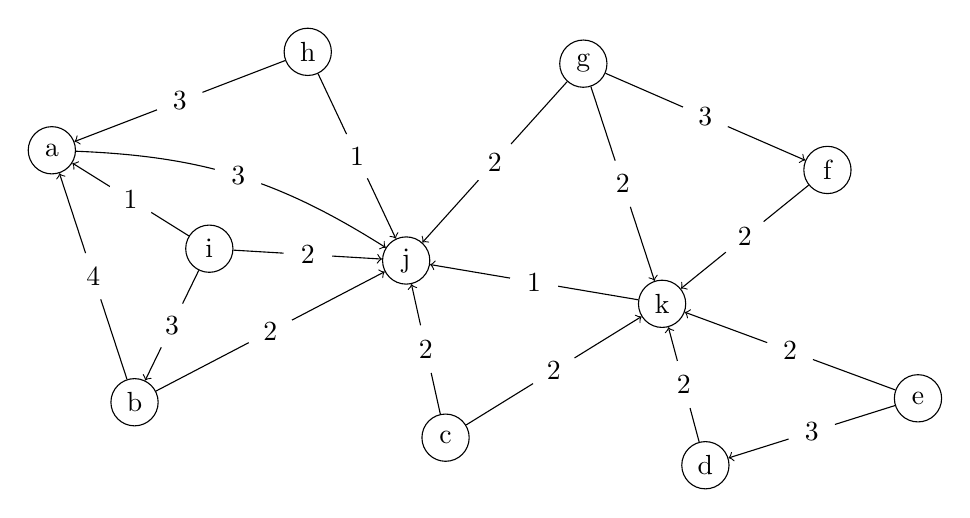
\begin{tikzpicture}
    % Nodes
    \node[circle, draw, minimum size=0.6cm, inner sep=0pt] at (0.5* 0.0, 0.5* 8.5) (a) {a};
    \node[circle, draw, minimum size=0.6cm, inner sep=0pt] at (0.5* 2.1, 0.5* 2.1) (b) {b};
    \node[circle, draw, minimum size=0.6cm, inner sep=0pt] at (0.5* 10.0, 0.5* 1.2) (c) {c};
    \node[circle, draw, minimum size=0.6cm, inner sep=0pt] at (0.5* 16.6, 0.5* 0.5) (d) {d};
    \node[circle, draw, minimum size=0.6cm, inner sep=0pt] at (0.5* 22.0, 0.5* 2.2) (e) {e};
    \node[circle, draw, minimum size=0.6cm, inner sep=0pt] at (0.5* 19.7, 0.5* 8.0) (f) {f};
    \node[circle, draw, minimum size=0.6cm, inner sep=0pt] at (0.5* 13.5, 0.5* 10.7) (g) {g};
    \node[circle, draw, minimum size=0.6cm, inner sep=0pt] at (0.5* 6.5, 0.5* 11.0) (h) {h};
    \node[circle, draw, minimum size=0.6cm, inner sep=0pt] at (0.5* 4.0, 0.5* 6.0) (i) {i};
    \node[circle, draw, minimum size=0.6cm, inner sep=0pt] at (0.5* 9.0, 0.5* 5.7) (j) {j};
    \node[circle, draw, minimum size=0.6cm, inner sep=0pt] at (0.5* 15.5, 0.5* 4.6) (k) {k};

    \draw[->] (a) edge[bend left=15] node[circle, fill=white] {3} (j);

    \draw[->] (b) edge node[circle, fill=white] {4} (a);
    \draw[->] (b) edge node[circle, fill=white] {2} (j);

    \draw[->] (c) edge node[circle, fill=white] {2} (j);
    \draw[->] (c) edge node[circle, fill=white] {2} (k);

    \draw[->] (d) edge node[circle, fill=white] {2} (k);

    \draw[->] (e) edge node[circle, fill=white] {3} (d);
    \draw[->] (e) edge node[circle, fill=white] {2} (k);

    \draw[->] (f) edge node[circle, fill=white] {2} (k);

    \draw[->] (g) edge node[circle, fill=white] {3} (f);
    \draw[->] (g) edge node[circle, fill=white] {2} (j);
    \draw[->] (g) edge node[circle, fill=white] {2} (k);

    \draw[->] (h) edge node[circle, fill=white] {3} (a);
    \draw[->] (h) edge node[circle, fill=white] {1} (j);

    \draw[->] (i) edge node[circle, fill=white] {1} (a);
    \draw[->] (i) edge node[circle, fill=white] {3} (b);
    \draw[->] (i) edge node[circle, fill=white] {2} (j);

    \draw[->] (k) edge node[circle, fill=white] {1} (j);
  \end{tikzpicture}
  \caption{Upward-Graph des Beispielgraphs}
  \label{ch::fig::upward_graph}
\end{figure}

Die Definition des Downward-Graphens erfolgt nun analog zu der des Upward-Graphens:

\begin{definition}[Downward-Graph]
  Sei $G = (V, E)$ und eine vertex-to-level-Funktion dazu gegeben. Dann ist ein Upward-Graph des transponierten Graphens $G^T$ ein \emph{Downward-Graph} zu $G$.
\end{definition}

Ist ein Graph ungerichtet, so ist er äquivalent zu seinem transponierten Graphen, daher sind dann sind auch Upward- und Downward-Graph äquivalent.
\autoref{ch::fig::upward_graph} entspricht somit gleichzeitig dem Downward-Graph des Beispielgraphens aus \autoref{graphs:fig:beispielgraph}.
Es ist zu zeigen, dass Anfragen auf einem auf diese Art definierten Contracted-Graph $C = (G_u, G_d)$ ebenfalls korrekt sind.

\begin{beweis}[Korrektheit Contracted-Graph Anfrage]
  Da sowohl im Upward- als auch im Downward-Graphen nur Kanten existieren, deren Gewicht mindestens dem kürzesten Pfad Abstand der verbundenen Knoten entspricht, kann in $C$ kein Pfad gefunden werden, der nicht auch in $G$ existiert.

  Sei ${sp}_G(s, t)$ der kürzeste $s$-$t$-Pfad auf $G$ der unter allen kürzesten $s$-$t$-Pfaden den Knoten $m$ mit dem höchsten Level enthält.
  Erstelle aus diesem Pfad $(s, \dotsc, t)$ zwei Pfade: $(s, \dotsc, m)$ und $(t, \dotsc, m)$.
  Betrachte den Teilpfad $(s, \dotsc, m)$ der Hop-Länge $n_s$.

  Finde nun den ersten Knoten $s'$ nach $s$, für den gilt, dass sein Level größer als das von $s$ ist und zwischen denen auf allen Pfaden nur Knoten kleiner Level liegen.
  Für diesen gibt es nach der Definition des Upward-Graphen eine Kante $(s, s')$ mit optimalem Gewicht.
  Wiederhole dies für den Teilpfad $(s', \dotsc, m)$, bis $s' = m$.
  Durch diese Kanten lässt sich $m$ von $s$ aus in $C$ mit optimaler Distanz finden.

  Analog wird für den Teilpfad $(t, \dotsc, m)$ im Downward-Graphen argumentiert.
  \qed
\end{beweis}

Dass nur Kanten $(t, h)$ erstellt werden müssen, wenn $h$ das größte und $t$ das zweitgrößte Level auf allen $t$-$h$-Pfaden hat, ist in \autoref{fig:people:notwendige_kanten} veranschaulicht.
Die Zahl unter dem Knotennamen entspricht dabei dem Level des Knotens.
Es muss keine $(u, w)$ Kante erstellt werden, da $w$ über $v$ erreicht werden kann.

\begin{figure}[h!]
  \centering
  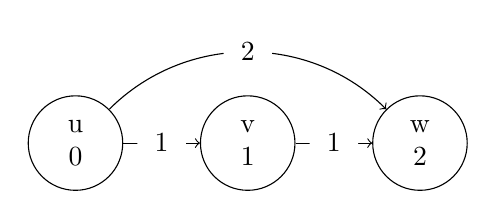
\begin{tikzpicture}[scale=1.75]
    \node[circle, draw, minimum size=1.2cm, inner sep=0pt , align=center] at (0*1.25, 0) (u) {u\\0};
    \node[circle, draw, minimum size=1.2cm, inner sep=0pt , align=center] at (1*1.25, 0) (v) {v\\1};
    \node[circle, draw, minimum size=1.2cm, inner sep=0pt , align=center] at (2*1.25, 0) (w) {w\\2};

    \draw[->] (u) edge[bend left=45] node[circle, fill=white] {2} (w);
    \draw[->] (u) edge node[circle, fill=white] {1} (v);
    \draw[->] (v) edge node[circle, fill=white] {1} (w);
  \end{tikzpicture}
  \caption{Beispiel für notwendige Kanten im Upward-Graph}
  \label{fig:people:notwendige_kanten}
\end{figure}

\subsection{Kontraktion erfüllt diese Definition}

Bei der Knoten-Kontraktion des Knotens $v$ wird für den Vorgänger-Nachfolger-Pfad $(u, v, w)$ eine Abkürzung eingefügt, wenn dies der einzige kürzeste $u$-$w$-Pfad ist.
Ist dies der Fall, dann sind die Knoten aller andern kürzesten Pfade zuvor bereits kontrahiert worden und haben ein niedrigeres Level als $u$ und $w$.
Deswegen bilden diese Abkürzungen mitsamt den Kanten des ursprünglichen Graphen die Kantenmenge des Upward- und Downward-Graphen (nach der neuen Definition \ref{people:def:upward_graph}), wobei die Zuordnung zu Downward- und Upward-Graph durch die Reihenfolge der Kontraktion von $u$ und $w$ definiert ist.

Wenn die Kontraktionsbedingung abgeschwächt wird, werden nicht notwendige und nicht optimale Kanten eingefügt, dies lässt die Definition aber zu.
Daher entspricht ein durch Graphen-Kontraktion erzeugter Graph der neuen Definition.

\subsection{Algorithmus}

Da das Berechnen aller kürzesten Pfade zwischen zwei Knoten aufwendig ist, wird die Bedingung zum Hinzufügen einer Kante bei der Berechnung eines Contracted-Graphens vereinfacht.
Es werden $(t, h)$-Kanten eingefügt, sobald ein optimaler $t$-$h$-Pfad gefunden wurde, auf dem $h$ das größte und $t$ das zweitgrößte Level hat.
Dies ist hinreichend, fügt im Zweifel jedoch mehr Kanten als notwendig ein.

Um einen Upward-Graphen zu berechnen, wird für jeden Knoten $t \in V$ eine angepasste Dijkstra-Suche ausgeführt, bei der für jeden Knoten jeweils notiert wird, was das größte Level auf dem Pfad zur Wurzel ist.
Diese Information kann mit der \emph{max-on-path} Funktion ${mop}$ abgerufen werden.
Ein Knoten $h \in V$, $h \neq t$ ist dabei der Kopf einer Upward-Graph Kante, für die ${mop}(h) = {vtl}(h)$ und ${mop}({pre}(h)) = {vtl}(t)$ gilt.
Das Gewicht der Kante wird der Dijkstra-Suche entnommen.
Die Suche kann abgebrochen werden, wenn für alle nicht-expandierten Knoten $h$ die Bedingung ${mop}({pre}(h)) > {vtl}(h)$ erfüllt ist.
Ist dies erfüllt, so hat die Wurzel $t$ auf dem $t$-$h$-Pfad nicht das zweitgrößte Level und damit kann $h$ nicht der Kopf einer Upward-Kante sein.
\autoref{ch:fig:ch_brute_force_suchbaum} zeigt dies für den Knoten $a$ im Beispielgraphen.
Die linke Zahl steht dabei für das Level des jeweiligen Knotens, die rechte Zahl für das größte Level auf dem Pfad zur Wurzel.

\begin{figure}[h!]
  \centering
  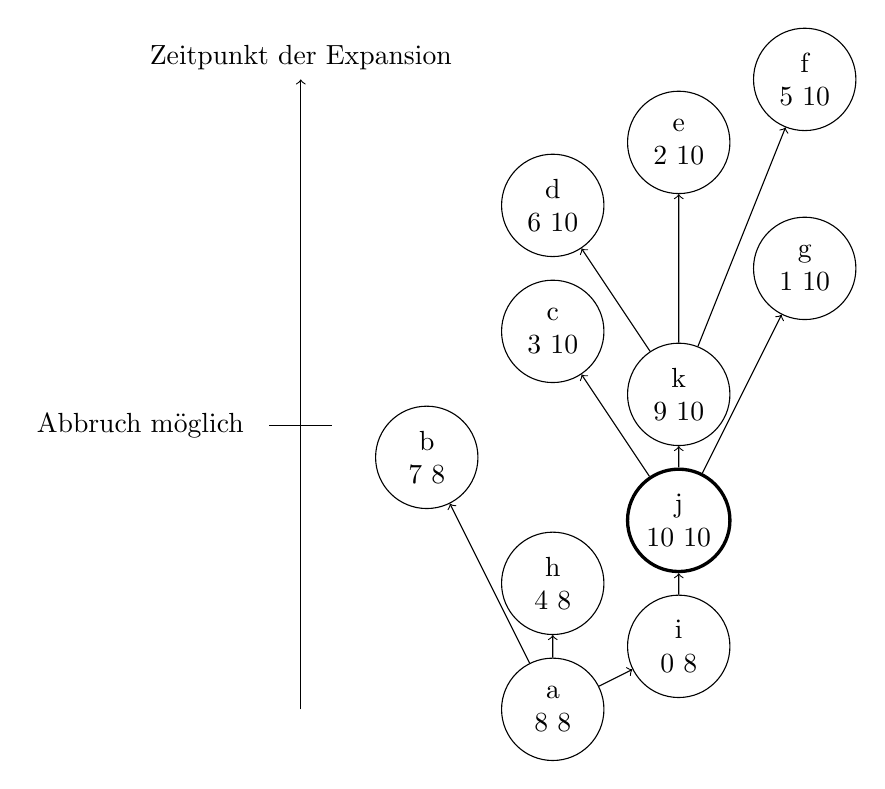
\begin{tikzpicture}[scale=0.8]
    % Nodes
    % a & b & c & d & e & f & g & h & i & j & k &
    % 8 & 7 & 3 & 6 & 2 & 5 & 1 & 4 & 0 & 10 & 9 &

    \node[circle, draw, minimum size=1.3cm, inner sep=0pt , align=center] at (2* 1, 0) (a) {a\\8 8};
    \node[circle, draw, minimum size=1.3cm, inner sep=0pt , align=center] at (2* 0, 4) (b) {b\\7 8};
    \node[circle, draw, minimum size=1.3cm, inner sep=0pt , align=center] at (2* 1, 6) (c) {c\\3 10};
    \node[circle, draw, minimum size=1.3cm, inner sep=0pt , align=center] at (2* 1, 8) (d) {d\\6 10};
    \node[circle, draw, minimum size=1.3cm, inner sep=0pt , align=center] at (2* 2, 9) (e) {e\\2 10};
    \node[circle, draw, minimum size=1.3cm, inner sep=0pt , align=center] at (2* 3, 10) (f) {f\\5 10};
    \node[circle, draw, minimum size=1.3cm, inner sep=0pt , align=center] at (2* 3, 7) (g) {g\\1 10};
    \node[circle, draw, minimum size=1.3cm, inner sep=0pt , align=center] at (2* 1, 2) (h) {h\\4 8};
    \node[circle, draw, minimum size=1.3cm, inner sep=0pt , align=center] at (2* 2, 1) (i) {i\\0 8};
    \node[circle, draw, minimum size=1.3cm, inner sep=0pt , align=center, very thick] at (2* 2, 3) (j) {j\\10 10};
    \node[circle, draw, minimum size=1.3cm, inner sep=0pt , align=center] at (2* 2, 5) (k) {k\\9 10};

    \draw[->] (a) edge (b);
    \draw[->] (a) edge (h);
    \draw[->] (a) edge (i);
    \draw[->] (j) edge (c);
    \draw[->] (i) edge (j);
    \draw[->] (k) edge (d);
    \draw[->] (j) edge (k);
    \draw[->] (k) edge (e);
    \draw[->] (k) edge (f);
    \draw[->] (j) edge (g);

    \draw[->] (-2, 0) -- (-2, 10) node[above] {Zeitpunkt der Expansion};

    \draw (-2.5, 4.5) -- (-1.5, 4.5) node[left=1cm] {Abbruch möglich};

  \end{tikzpicture}
  \caption{Contracted-Graph PEOPLE Suchbaum}
  \label{ch:fig:ch_brute_force_suchbaum}
\end{figure}

Die Information des größten Levels auf dem Pfad zur Wurzel kann dabei beim Update eines Knotens übertragen werden, indem das Maximum des bisherigen größten Levels und das Level des upgedateten Knotens gebildet wird.


Die Abbruchbedingung kann durch Betrachtung einer Menge an \emph{lebendigen Knoten} verfolgt werden.
Sobald diese keine Knoten mehr enthält, kann die Suche abgebrochen werden.
Zu Beginn ist nur der Startknoten lebendig, die Lebendigkeit wird dann jeweils an die Kinder vererbt.
Ein Knoten stirbt, nachdem er expandiert worden ist oder wenn er den Kopf einer Upward-Graph Kante bildet.
In dem Beispiel in \autoref{ch:fig:ch_brute_force_suchbaum} wäre dies etwa nach der Expansion von $b$ der Fall.
Bei einer \emph{guten} vertex-to-level-Funktion kann davon ausgegangen werden, dass viele Suchen früh abgebrochen werden können.

Die Berechnung ist \emph{embarrassingly parallel}, jeder Knoten kann unabhängig von den anderen berechnet werden.
Der textuell beschriebene Algorithmus ist im Algorithmus \ref{alg:people:ch} dargestellt und wird Contracted-Graph PEOPLE Algorithmus genannt.

\begin{algorithm}[p]
  \caption{CH-PEOPLE}
  \begin{algorithmic}[1]
    \Require Graph $G = (V, E)$, vertex-to-level Funktion ${vtl}$, Knoten $s \in V$
    \Ensure $E_s$
    \State // Initialisiere Distanz- und Vorgänger-Funktion
    \ForAll{$v \in V$}
    \State ${dist}(v) \leftarrow \infty$
    \State ${pre}(v) \leftarrow {none}$
    \EndFor

    \State
    \State // Initialisiere Suche
    \State ${dist}(s) \leftarrow 0$
    \State $Q\leftarrow \{ s \}$
    \State ${pre}(s) \leftarrow s$

    \State
    \State // Initialisiere max-on-path
    \State ${mop}(s) \leftarrow {vtl}(s)$
    \State $E_s \leftarrow \{ \}$
    \State ${alive} \leftarrow \{ s \}$

    \State
    \While{$Q \neq \emptyset \land {alive} \neq \emptyset$}
    \State $u \leftarrow{extract\_min}(Q)$\label{graphs:dijkstra:pop}

    \State
    \State // Baue Kantenmenge
    \If {$u \neq s \land {mop}(u) = {vtl}(u)$}
    \State $E_s \leftarrow E_s \cup \{ (s, u, {dist}(u)) \}$
    \State ${alive} \leftarrow {alive} \setminus \{ u \}$
    \EndIf

    \State
    \State // Aktualisiere Nachbarn
    \ForAll{$(u, v, w) \in E$}
    \If {${dist}(u) + w < {dist}(v)$}
    \State ${dist}(v) \leftarrow {dist}(u) + w$
    \State ${pre}(u) \leftarrow v$
    \State $Q = Q \cup \{ v \}$
    \State
    \State // setze max\_level\_path
    \State ${mop}(v) \leftarrow \max({mop}(v), {vtl}(v))$
    \State
    \If {$u \in {alive}$}
    \State ${alive} \leftarrow {alive} \cup \{ v \}$
    \EndIf
    \EndIf
    \EndFor

    \State ${alive} \leftarrow {alive} \setminus \{ u \}$

    \EndWhile

    \State
    \State \Return $E_s$
  \end{algorithmic}
  \label{alg:people:ch}
\end{algorithm}

\subsection{Änderung von Kantengewichten}

Bei Graphen mit hierarchischer Struktur und einer guten vertex-to-Level-Funktion ist anzunehmen, dass die Suche nach Algorithmus \ref{alg:people:ch}  in den meisten Fällen früh abbricht.
Dies ist einerseits für die Effizienz der Berechnung von Vorteil, verdeutlicht aber auch, dass für die Bestimmung der ausgehenden Kanten des Contracted-Graphen für viele Knoten jeweils nur ihre lokale Umgebung von Bedeutung ist, wobei insbesondere Knoten mit einem hohen Level hierbei eine Ausnahme bilden.
Änderungen der Kantengewichte außerhalb dieser Umgebung haben daher für viele Knoten keinen Einfluss auf den Suchbaum des Algorithmus \ref{alg:people:ch}.

Diese Eigenschaft lässt sich nutzen, um nach einer Änderung der Kantengewichte nicht für jeden Knoten sämtliche ausgehenden Kanten neu berechnen zu müssen.
Zwei mögliche Ansätze bieten sich hierfür an:
Zum einen könnte für jeden Knoten gespeichert werden, von welchen Kanten er beeinflusst wird.
Zum anderen könnte für eine geänderte Kante berechnet werden, welche Knoten von ihr beeinflusst werden.

Das Speichern des Bereichs, der einen Knoten beeinflusst, kann in Graphen in der euklidischen Ebene beispielsweise durch Bounding-Boxen realisiert werden.
Ob es eine effiziente Methode gibt, mit der der Einflussbereich einer Kante bestimmt werden kann, wird in dieser Arbeit nicht behandelt.

\subsection{Abkürzungsproblem}

Es liegt nahe, als abgekürzten Knoten denjenigen Knoten mit dem dritthöchsten Level auszuwählen und sich darauf zu verlassen, dass die Suche von diesem aus die nächste Abkürzung findet, da dies der Knoten-Kontraktion entspricht.
Das ist praktisch, da dann jede Abkürzung nur einmal erstellt werden muss, dafür muss jedoch gelten, dass die Vorwärtssuche für $s$-$t$ den gleichen Pfad findet wie die Rückwärtssuche (die Suche auf dem transponierten Graphen) für $t$-$s$.
Dies ist nicht garantiert, wenn als Graph eine Datenstruktur verwendet wird, welche die Nachbarn nicht in einer definierten Ordnung ausgibt (etwa eine HashMap).
Eine nicht stabile Prioritätswarteschlange hat ebenfalls den gleichen Effekt.

\autoref{ch:fig:problem_shortcut} zeigt ein solches Szenario.
Im Contracted-Graphen $C$ wurde der $a$-$e$-Pfad $(a, e)$ gefunden, dessen Abkürzungen nun ersetzt werden.
Zunächst wird für die Abkürzung $(a, e)$ der abgekürzte Knoten $d$ gefunden, was zu dem Pfad $(a, d, e)$ führt.
Es wird darauf vertraut, dass die Suche von $d$ aus die Abkürzung $(d, a)$ mit dem Knoten $b$ findet, jedoch geschieht dies nicht, wenn $a$ von $d$ aus über $c$ erreicht wird.

\begin{figure}[h!]
  \centering
  \begin{subfigure}[b]{0.49\textwidth}
    \centering
    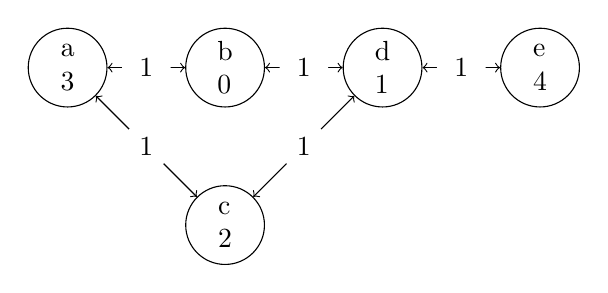
\begin{tikzpicture}
      % Nodes
      \node[circle, draw, minimum size=1cm, inner sep=0pt, align=left] at (2*0, 2*0) (a) {a\\3};
      \node[circle, draw, minimum size=1cm, inner sep=0pt, align=left] at (2*1, 2*0) (b) {b\\0};
      \node[circle, draw, minimum size=1cm, inner sep=0pt, align=left] at (2*1, 2*-1) (c) {c\\2};
      \node[circle, draw, minimum size=1cm, inner sep=0pt, align=left] at (2*2, 2*0) (d) {d\\1};
      \node[circle, draw, minimum size=1cm, inner sep=0pt, align=left] at (2*3, 2*0) (e) {e\\4};

      \draw[<->] (a) edge node[circle, fill=white] {1} (b);
      \draw[<->] (b) edge node[circle, fill=white] {1} (d);
      \draw[<->] (d) edge node[circle, fill=white] {1} (e);

      \draw[<->] (a) edge node[circle, fill=white] {1} (c);
      \draw[<->] (c) edge node[circle, fill=white] {1} (d);
    \end{tikzpicture}
    \caption{Graph}
  \end{subfigure}
  \hfill
  \begin{subfigure}[b]{0.49\textwidth}
    \centering
    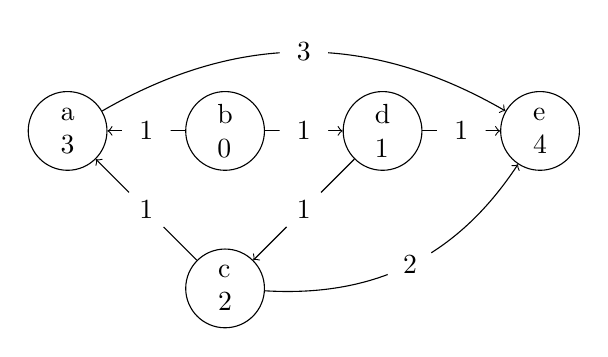
\begin{tikzpicture}
      % Nodes
      \node[circle, draw, minimum size=1cm, inner sep=0pt, align=left] at (2*0, 2*0) (a) {a\\3};
      \node[circle, draw, minimum size=1cm, inner sep=0pt, align=left] at (2*1, 2*0) (b) {b\\0};
      \node[circle, draw, minimum size=1cm, inner sep=0pt, align=left] at (2*1, 2*-1) (c) {c\\2};
      \node[circle, draw, minimum size=1cm, inner sep=0pt, align=left] at (2*2, 2*0) (d) {d\\1};
      \node[circle, draw, minimum size=1cm, inner sep=0pt, align=left] at (2*3, 2*0) (e) {e\\4};

      \draw[<-] (a) edge node[circle, fill=white] {1} (b);
      \draw[->] (b) edge node[circle, fill=white] {1} (d);
      \draw[->] (d) edge node[circle, fill=white] {1} (e);

      \draw[->] (c) edge node[circle, fill=white] {1} (a);
      \draw[<-] (c) edge node[circle, fill=white] {1} (d);

      \draw[->] (c) edge[bend right] node[circle, fill=white] {2} (e);
      \draw[->] (a) edge[bend left] node[circle, fill=white] {3} (e);
    \end{tikzpicture}
    \caption{Upward- und Downard-Graph von $C$}
  \end{subfigure}
  \begin{subfigure}[b]{0.49\textwidth}
    \centering
    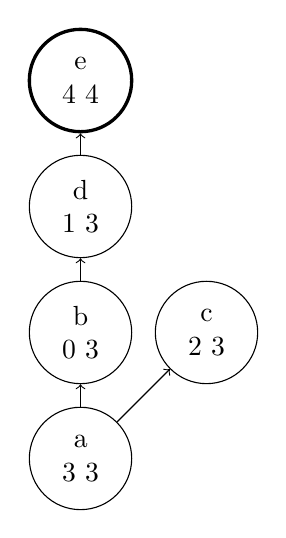
\begin{tikzpicture}[scale=0.8]
      % Nodes
      \node[circle, draw, minimum size=1.3cm, inner sep=0pt, align=center] at (2*0, 2*0) (a) {a\\3 3};
      \node[circle, draw, minimum size=1.3cm, inner sep=0pt, align=center] at (2*0, 2*1) (b) {b\\0 3};
      \node[circle, draw, minimum size=1.3cm, inner sep=0pt, align=center] at (2*1, 2*1) (c) {c\\2 3};
      \node[circle, draw, minimum size=1.3cm, inner sep=0pt, align=center] at (2*0, 2*2) (d) {d\\1 3};
      \node[circle, draw, minimum size=1.3cm, inner sep=0pt, align=center, very thick] at (2*0, 2*3) (e) {e\\4 4};

      \draw[->] (a) edge node[] {} (b);
      \draw[->] (b) edge node[] {} (d);
      \draw[->] (d) edge node[] {} (e);
      \draw[->] (a) edge node[] {} (c);
    \end{tikzpicture}
    \caption{Suchbaum von $a$}
  \end{subfigure}
  \hfill
  \begin{subfigure}[b]{0.49\textwidth}
    \centering
    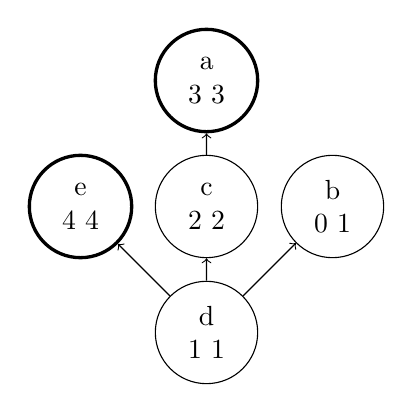
\begin{tikzpicture}[scale=0.8]
      % Nodes
      \node[circle, draw, minimum size=1.3cm, inner sep=0pt, align=center, very thick] at (2*1, 2*2) (a) {a\\3 3};
      \node[circle, draw, minimum size=1.3cm, inner sep=0pt, align=center] at (2*2, 2*1) (b) {b\\0 1};
      \node[circle, draw, minimum size=1.3cm, inner sep=0pt, align=center] at (2*1, 2*1) (c) {c\\2 2};
      \node[circle, draw, minimum size=1.3cm, inner sep=0pt, align=center] at (2*1, 2*0) (d) {d\\1 1};
      \node[circle, draw, minimum size=1.3cm, inner sep=0pt, align=center, very thick] at (2*0, 2*1) (e) {e\\4 4};

      \draw[->] (d) edge node[] {} (e);
      \draw[->] (d) edge node[] {} (c);
      \draw[->] (d) edge node[] {} (b);
      \draw[->] (c) edge node[] {} (a);
    \end{tikzpicture}
    \caption{Suchbaum von $d$}
  \end{subfigure}
  \caption{Problem beim Shortcut erstellen}
  \label{ch:fig:problem_shortcut}
\end{figure}

Für dieses Problem gibt es zwei Lösungen:
Für jede Abkürzung $(t, h)$ werden alle weiteren Abkürzungen die benötigt werden, um aus $(t, h)$ einen Pfad auf $G$ zu erstellen, gesammelt.
Dadurch werden viele Abkürzungen mehrfach erstellt, da eine Abkürzung Teil einer anderen Abkürzung sein kann.
Dies muss daher zwischen den einzelnen CH-PEOPLE Suchen synchronisiert werden, um den Speicherverbrauch zu minimieren.

Alternativ kann die Prioritätswarteschlange modifiziert werden, indem eine Totalordnung der Knoten bestimmt, in welcher Reihenfolge Knoten gleicher Distanz expandiert werden.

\section{PEOPLE}

Analog zur neuen Definition des Contracted-Graph lässt sich auch der Hub-Graph neu definieren.
Die dafür verwendete Definition des Forward-Labels weicht nur leicht von der des Upward-Graphen ab, lediglich die Anforderung, dass der Fuß einer Kante das zweitgrößte Level hat, entfällt.

\begin{definition}[Forward-Label]
  Sei $G = (V, E)$ und eine vertex-to-level Funktion dazu gegeben.
  Dann ist $L_f (t) \subset V \times \mathbb{R}$ ein Forward-Label für einen Knoten $t$ in $G$, wenn gilt:

  \begin{itemize}
    \item
          $L_f (t)$ enthält nur Einträge $(h, d)$ mit $h \in V$ und $d \in \mathbb{R}$, für die es einen $t$-$h$ Pfad der Länge $d \geq {spd}_G (t, h)$ gibt, sodass auf ihm $h$ das größte Level hat.

    \item
          $L_f (t)$ enthält alle Einträge $(h, {spd}_G (t, h))$ mit $h \in V$, für die gilt, dass auf \emph{allen} $t$-$h$ Pfaden $h$ das größte Level hat.
  \end{itemize}
\end{definition}


Hierbei ist ein Backward-Label ein Forward-Label des transponierten Graphen $G^T$.
Die Korrektheit dieser Definition folgt direkt daraus, dass der Knoten mit dem höchsten Level auf einem Pfad im Forward- und Backward-Label liegt.

\subsection{Algorithmus}

Solche Labels können wieder durch Merging aus einem Contracted-Graph erstellt werden, jedoch folgt aus dieser Definition auch die Möglichkeit, das Label eines bestimmten Knotens zu berechnen.
Der dafür verwendete Algorithmus \ref{alg:people:people} erzeugt direkt ein gepruntes Label, da er aus einem Dijkstra-Suchbaum auf $G$ das Label erzeugt und dieser nur optimale Distanzen enthält.
Da er für eine vorgegebene vertex-to-level-Funktion geprunte Label liefert, wird dieser Algorithmus PEOPLE, für \textbf{P}r\textbf{E}determined \textbf{O}rder, \textbf{P}runed \textbf{L}ab\textbf{e}l, genannt.

Ein Beispiel einer solchen Suche ist in \autoref{ch:fig:hl_brute_force_suchbaum} gezeichnet.
Das Label für $a$ enthält $j$, $f$ und $a$ selbst, da ihr Level das jeweils größte auf dem Pfad zur Wurzel ist.

\begin{figure}[h!]
  \centering
  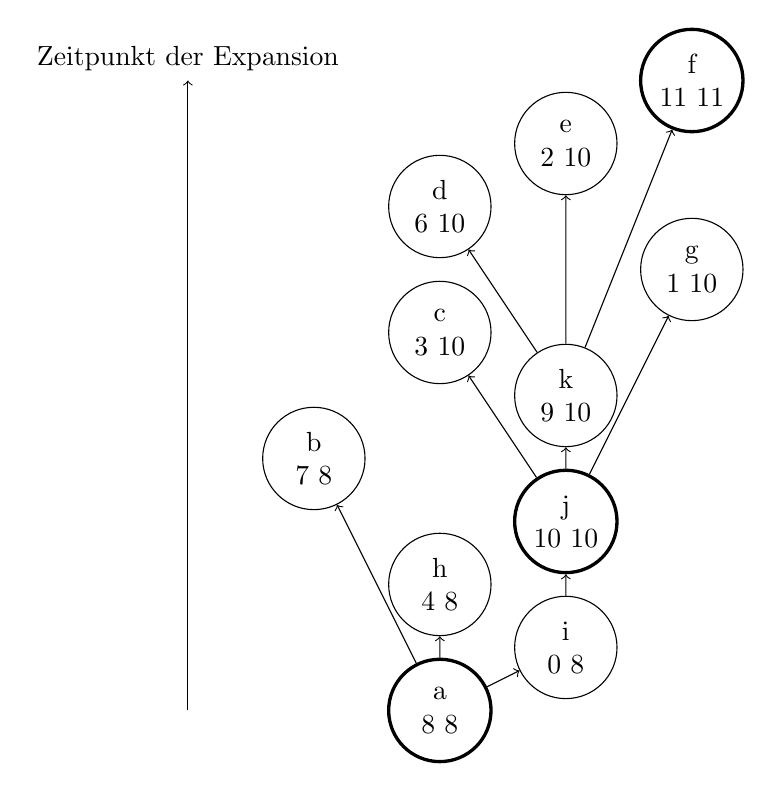
\begin{tikzpicture}[scale=0.8]
    % Nodes
    % a & b & c & d & e & f & g & h & i & j & k &
    % 8 & 7 & 3 & 6 & 2 & 5 & 1 & 4 & 0 & 10 & 9 &

    \node[circle, draw, minimum size=1.3cm, inner sep=0pt , align=center, very thick] at (2* 1, 0) (a) {a\\8 8};
    \node[circle, draw, minimum size=1.3cm, inner sep=0pt , align=center] at (2* 0, 4) (b) {b\\7 8};
    \node[circle, draw, minimum size=1.3cm, inner sep=0pt , align=center] at (2* 1, 6) (c) {c\\3 10};
    \node[circle, draw, minimum size=1.3cm, inner sep=0pt , align=center] at (2* 1, 8) (d) {d\\6 10};
    \node[circle, draw, minimum size=1.3cm, inner sep=0pt , align=center] at (2* 2, 9) (e) {e\\2 10};
    \node[circle, draw, minimum size=1.3cm, inner sep=0pt , align=center, very thick] at (2* 3, 10) (f) {f\\11 11};
    \node[circle, draw, minimum size=1.3cm, inner sep=0pt , align=center] at (2* 3, 7) (g) {g\\1 10};
    \node[circle, draw, minimum size=1.3cm, inner sep=0pt , align=center] at (2* 1, 2) (h) {h\\4 8};
    \node[circle, draw, minimum size=1.3cm, inner sep=0pt , align=center] at (2* 2, 1) (i) {i\\0 8};
    \node[circle, draw, minimum size=1.3cm, inner sep=0pt , align=center, very thick] at (2* 2, 3) (j) {j\\10 10};
    \node[circle, draw, minimum size=1.3cm, inner sep=0pt , align=center] at (2* 2, 5) (k) {k\\9 10};

    \draw[->] (a) edge (b);
    \draw[->] (a) edge (h);
    \draw[->] (a) edge (i);
    \draw[->] (j) edge (c);
    \draw[->] (i) edge (j);
    \draw[->] (k) edge (d);
    \draw[->] (j) edge (k);
    \draw[->] (k) edge (e);
    \draw[->] (k) edge (f);
    \draw[->] (j) edge (g);

    \draw[->] (-2, 0) -- (-2, 10) node[above] {Zeitpunkt der Expansion};

  \end{tikzpicture}
  \caption{Hub-Graph PEOPLE Suchbaum}
  \label{ch:fig:hl_brute_force_suchbaum}
\end{figure}

\begin{algorithm}[p]
  \caption{PEOPLE}
  \begin{algorithmic}[1]
    \Require Graph $G = (V, E)$, vertex-to-level Funktion ${vtl}$, Knoten $s \in V$
    \Ensure $L_f (s)$
    \State // Initialisiere Distanz- und Vorgänger-Funktion
    \ForAll{$v \in V$}
    \State ${dist}(v) \leftarrow \infty$
    \State ${pre}(v) \leftarrow {none}$
    \EndFor

    \State
    \State // Initialisiere Suche
    \State ${dist}(s) \leftarrow 0$
    \State $Q\leftarrow \{ s \}$
    \State ${pre}(s) \leftarrow s$

    \State
    \State // Initialisiere max-on-path
    \State ${mop}(s) \leftarrow {vtl}(s)$
    \State $L_f (s) \leftarrow \{ \}$

    \State
    \While{$Q \neq \emptyset$}
    \State $u \leftarrow{extract\_min}(Q)$

    \State
    \State // Baue Label
    \If {${mop}(u) = {vtl}(u)$}
    \State $L_f (s) \leftarrow L_f (s) \cup \{ (u, {dist}(u)) \}$
    \EndIf

    \State
    \State // Aktualisiere Nachbarn
    \ForAll{$(u, v, w) \in E$}
    \If {${dist}(u) + w < {dist}(v)$}
    \State ${dist}(v) \leftarrow {dist}(u) + w$
    \State ${pre}(u) \leftarrow v$
    \State $Q = Q \cup \{ v \}$
    \State
    \State // setze max\_level\_path
    \State ${mop}(v) \leftarrow \max({mop}(v), {vtl}(v))$
    \EndIf
    \EndFor

    \EndWhile

    \State
    \State \Return $L_f (s)$
  \end{algorithmic}
  \label{alg:people:people}
\end{algorithm}

\subsection{Größe der Label}\label{subsection:people:label_size}

Die mit PEOPLE erzeugten Labels können mitunter kleiner sein, als durch Merging erzeugte Label.
Insbesondere kann das Merging von Contracted-Graphen, welche durch Graphen-Kontraktion erzeugt wurden, Labels erzeugen, die nicht minimal sind.

\autoref{fig:people:better_label_size} zeigt ein solches Beispiel, wobei die Zahl unter dem Namen des Knotens dem Level des Knotens entspricht.
Der Upward-Graph kann hierbei sowohl durch PEOPLE als auch durch Graphen-Kontraktion erstellt worden sein.
Nach der neuen Definition des Forward-Labels muss das Label von $c$ nur $d$ und $b$ enthalten.
Wird es aber durch Merging erzeugt, so enthält es auch $a$.
Dieses Verhalten tritt auf, wenn kürzeste Pfaden nicht eindeutig sind.
Daher ist anzunehmen, dass unter anderem in Grid-Graphen dieses Phänomen häufiger auftritt.

Um tatsächlich minimale Label zu erzeugen, muss der Algorithmus \ref{alg:people:people} verändert werden:
Kann ein Knoten $v$ über $u$ erreicht werden, aber die Kosten hierfür sind gleich groß wie bisher, so wird $u$ trotzdem als Vorgänger von $v$ gesetzt, wenn ${mop}(u) > {mop}(v)$.

\begin{figure}[h!]
  \begin{subfigure}[b]{0.49\textwidth}
    \centering
    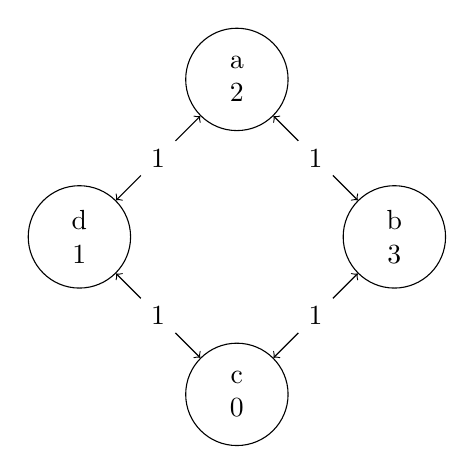
\begin{tikzpicture}[scale=1]
      % Nodes
      \node[circle, draw, minimum size=1.3cm, inner sep=0pt, align=center] at (2*1, 2*2) (a) {a\\2};
      \node[circle, draw, minimum size=1.3cm, inner sep=0pt, align=center] at (2*2, 2*1) (b) {b\\3};
      \node[circle, draw, minimum size=1.3cm, inner sep=0pt, align=center] at (2*1, 2*0) (c) {c\\0};
      \node[circle, draw, minimum size=1.3cm, inner sep=0pt, align=center] at (2*0, 2*1) (d) {d\\1};

      \draw[<->] (a) edge node[circle, fill=white] {1} (b);
      \draw[<->] (b) edge node[circle, fill=white] {1} (c);
      \draw[<->] (c) edge node[circle, fill=white] {1} (d);
      \draw[<->] (d) edge node[circle, fill=white] {1} (a);
    \end{tikzpicture}
    \caption{Graph}
  \end{subfigure}
  \hfill
  \begin{subfigure}[b]{0.49\textwidth}
    \centering
    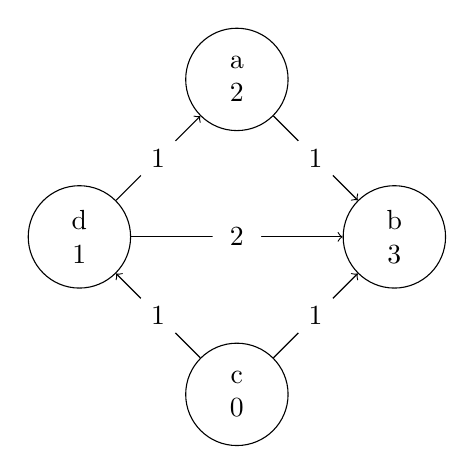
\begin{tikzpicture}[scale=1]
      % Nodes
      \node[circle, draw, minimum size=1.3cm, inner sep=0pt, align=center] at (2*1, 2*2) (a) {a\\2};
      \node[circle, draw, minimum size=1.3cm, inner sep=0pt, align=center] at (2*2, 2*1) (b) {b\\3};
      \node[circle, draw, minimum size=1.3cm, inner sep=0pt, align=center] at (2*1, 2*0) (c) {c\\0};
      \node[circle, draw, minimum size=1.3cm, inner sep=0pt, align=center] at (2*0, 2*1) (d) {d\\1};


      \draw[->] (c) edge node[circle, fill=white] {1} (d);
      \draw[->] (c) edge node[circle, fill=white] {1} (b);

      \draw[->] (d) edge node[circle, fill=white] {2} (b);
      \draw[->] (d) edge node[circle, fill=white] {1} (a);

      \draw[->] (a) edge node[circle, fill=white] {1} (b);
    \end{tikzpicture}
    \caption{Upward- und Downward-Graph}
  \end{subfigure}
  \caption{Beispiel für nicht-minimale Label}



  \label{fig:people:better_label_size}
\end{figure}

\subsection{Anwendungsgebiet}

Die Berechnung der Graphen-Kontraktion in Straßennetzwerken ist in vertretbarer Zeit möglich, jedoch gilt dies nicht für alle Graphklassen.
Insbesondere bei Graphen mit hohem durchschnittlichen Knotengrad stellt die Dijkstra-Suche für jeden Vorgänger einen signifikanten Kostenfaktor dar, sodass die Berechnung der Labels mittels PEOPLE effizienter sein kann.
Da die Labels parallel berechnet werden können, ist es durch den Einsatz geeigneter Hardware möglich, die Berechnungszeit zu verkürzen.

Der Algorithmus kann auch dazu verwendet werden, die Ergebnisse einer $s$-$t$-Anfrage effizient zu cachen.
Falls die Labels von $s$ und $t$ noch nicht vorhanden sind, werden sie generiert.
Nachfolgende Anfragen von $s$ oder nach $t$ können dann direkt auf die gespeicherten Labels zugreifen.

PEOPLE kann auch dafür benutzt werden, die durch eine vertex-to-level-Funktion induzierte durchschnittliche Label Größe anzugeben, ohne zuerst den Contracted-Graph und anschließend den Hub-Graphen zu berechnen.
Hierfür wird für $n \in \mathbb{N}$ Knoten das Label berechnet und über diese die durchschnittliche Größe der Labels angegeben.
Da sich dies leicht parallelisieren lässt, könnte in einem zukünftigen Schritt durch Optimierungsalgorithmen die Labelgrößen verkleinert werden.